\begin{figure*}[ht]
    \centering
    \includegraphics[width=0.9\textwidth, page=3]{images/tsne.pdf}
\caption{
t-SNE visualization of label embeddings based on different models.
% Same color denotes the labels (\eg, \textit{kid}, \textit{woman}) that belong to same major category like \textcolor[RGB]{158,1,66}{\textbf{Human}}.  
Same color denotes the labels (\eg, \textit{kid}, \textit{woman}) that belong to same major category like \textbf{Human} (in dark red).  
For Bert and VLP model, label embeddings are generated with the same manual template ``There is a \{label\} in the scene''. Compared with GloVe and Bert, VLP model can capture semantic and visual consistency among similar labels. (Best viewed in color.) 
    }
    \label{fig:labelemb}
\end{figure*}